\documentclass[10pt]{article}
\usepackage[T1]{fontenc}
\usepackage{lmodern,amsmath,amssymb,graphicx,hyperref}
\usepackage[margin=.74in]{geometry}
\setlength{\parindent}{0pt}\setlength{\parskip}{6pt}
\begin{document}
\begin{center}{\Large An exact finite test beyond the curve equation}\\[4pt]
17 November2026 --- local unsigned Lean evidence\end{center}
\textbf{Actual input and question.}
The previous fixed control constructs a nonzero polynomial $Q=E(v)$
from an actual72coefficient space and70full mixed-jet conditions.
Its kernel $\mathcal K$ enforces multiplicity four at a chosen target and
both signs at three other positions. The question is whether some
$Q$ in this kernel contains information beyond $Y^2-f(X)$.
Nonzero polynomial alone does not answer it.

\textbf{Actual restricted remainder.}
The existing monic-remainder linear map, restricted to $K$ scalars and
composed with $E$ and the actual kernel subtype, gives
\[
 T:\mathcal K\longrightarrow K[X][Y],\qquad
 T(v)=E(v)\bmod_{\rm monic}(Y^2-f(X)).
\]
The output has outer degree less than two, and its two outer coefficient
polynomials reconstruct it exactly. Its public evaluations vanish at the
stated target and pairs when their actual equations $y^2=f(x)$ hold.
This is point evaluation, not preservation of full ambient multiplicity
[pcc:unverified].

\textbf{Cubic coefficient bounds from the actual mask.}
Write $q_j$ for the constructed row polynomial, $0\le j<8$.
Actual coefficient recovery and the mask give
$\deg q_j\le15-2j$. Define the actual sums
\[
 A=\sum_{s=0}^3q_{2s}f^s,\qquad
 B=\sum_{s=0}^3q_{2s+1}f^s.
\]
An explicit quotient $D$, assembled from rows two through seven, satisfies
\[
 E(v)=C(A)+C(B)Y+(Y^2-C(f))D.
\]
The ring identity and outer degree less than two identify
$C(A)+C(B)Y$ with the actual monic remainder. No favorable quotient or
remainder is supplied as a premise [pcc:unverified].

For an explicit $f$ with $\deg f\le3$, each summand has degree at most
$15-s$ for $A$, or $13-s$ for $B$. Existing product, power and finite-sum
bounds therefore give
\[
 \deg A\le15,\qquad \deg B\le13.
\]
These bounds include zero rows; no nonzero leading coefficient or
cancellation assumption is hidden [pcc:unverified].

\textbf{The resulting exact finite test.}
Existing coefficient linear maps construct $R_f:K^{72}\to K^{30}$:
16coefficients of $A$ and14coefficients of $B$.
The degree bounds prove
\[
 R_f(v)=0\ \Longleftrightarrow\ T(v)=0
 \ \Longleftrightarrow\ (Y^2-f(X))\mid E(v),\qquad v\in\mathcal K.
\]
Thus a nonzero output would certify that the helper survives reduction
by the known curve equation. This work constructs the map and proves the
test; it does not yet prove such an output exists. Thirty is output
capacity, not rank [pcc:unverified].
\newpage
\begin{center}{\Large Evidence and the next actual image obligation}\end{center}
\begin{center}
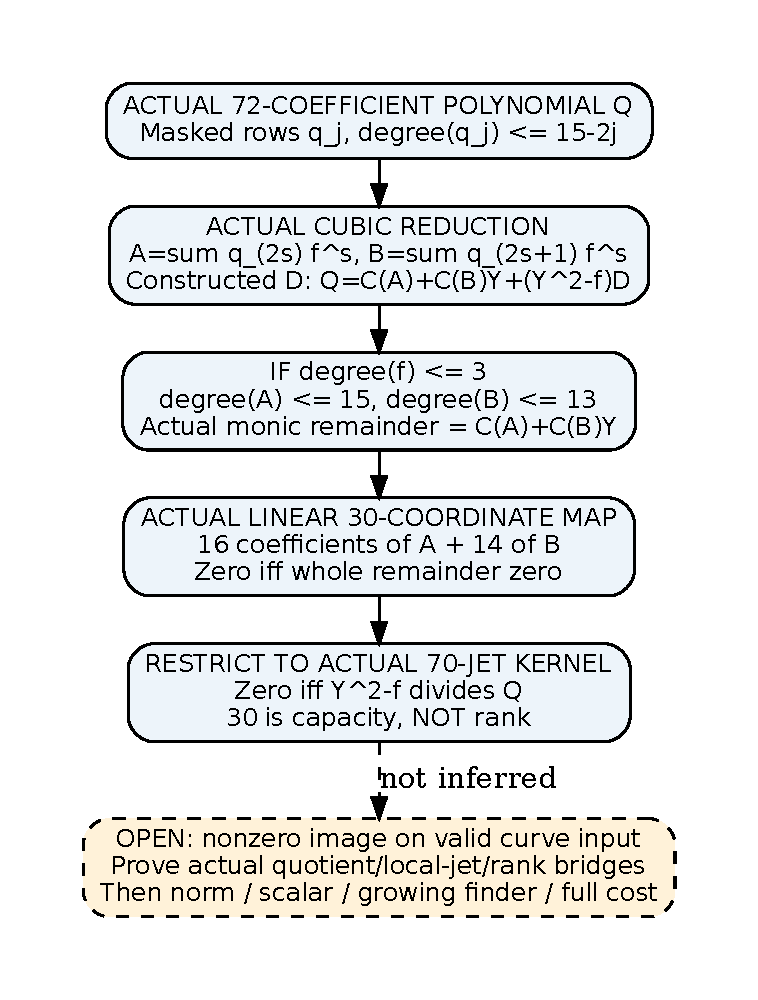
\includegraphics[width=.86\linewidth,height=3.65in,keepaspectratio]{remainder-dependencies-001.pdf}
\end{center}
\textbf{Exact proof map.}
\texttt{OrientationKernelCurveRemainder} supplies10new statements:
actual linear restriction, outer degree, reconstruction, zero criterion and
public evaluations. Source022/build023/receipt012 has77statements;
PCC-20261117-029281 [pcc:unverified].

\texttt{OrientationCubicRemainderBudget} supplies6new statements:
masked row degree, even/odd degree bounds, actual eight-row expansion,
quotient identity and \texttt{actual\_remainder}.
Source025/build026/receipt013 has83statements;
PCC-20261117-d0b6b1 [pcc:unverified].

\texttt{OrientationFiniteCurveCoordinates} supplies8new statements:
actual coefficient ports, finite zero-detection and kernel divisibility.
Source026/build027/receipt014 has91statements;
PCC-20261117-afecda [pcc:unverified].

All accepted runs exit0 without warnings. All91printed dependencies use
only standard \texttt{propext}, \texttt{Classical.choice} and
\texttt{Quot.sound}. Final91includes67committed parent and24new statements.
These are local unsigned records outside shared Transport53/57 audit/fresh.

\textbf{Next.}
Prove or refute a nonzero image of this actual restricted30coordinate map
under explicit valid, distinct, nonzero prime-field curve data.
A prospective route through the actual multiplicity-three quotient space
is recorded in protocol004; its degree, local multiplicity and rank
compatibilities remain unproved. Only after that image question comes
rational norm/scalar extraction and complete growing-family costs.

\textbf{Reproduction and sources.}
Maps012--014 and exclusive pre-calls pin the sources and dependencies.
Lean4.35.0 uses default limits. Failed021/023/024sources and all raw outputs
remain. No native/paid/attack/timing/scaling campaign or old proof replay.
Prior frozen graphs/reports stay exact; this is their versioned continuation.
No speed dashboard change. Protected PCC divergence prevents publication;
no history rewrite or watcher change.
Mathlib RingDivision/Div/OfFn and coefficient/degree/linear-map laws are used
as stated. Primary
\href{https://doi.org/10.1109/TIT.2013.2243800}{Beelen et al2013, Theorem6/(2)}
read scope remains in literature-review001. KB unavailable; no novelty claim.
\end{document}
